\documentclass[conference]{IEEEtran}
\usepackage{amsmath,amssymb}
\usepackage{booktabs}
\usepackage{graphicx}
\graphicspath{{figures/}{./}{reports/figures/}}
\usepackage{cite}
\usepackage{url}
% NOTE (team): check every reference against the original paper before submission.
% Least certain: heimes2008rnn, babu2016cnn, zheng2017lstm, li2018cnn.

\begin{document}

\title{Remaining Useful Life Prediction for Industrial Engines:\\
Sequence Models and a Hybrid on NASA C-MAPSS}

\author{\IEEEauthorblockN{Kush Puri, Aadit Vachher, Vachan Gupta, Aabir Sarkar, Kushagra Maheshwari}
\IEEEauthorblockA{Team T017, CSAI, Rishihood University}}

\maketitle

\begin{abstract}
In the first phase of this project, a Random Forest on 57 hand-engineered degradation features predicted the Remaining Useful Life (RUL) of turbofan engines in the NASA C-MAPSS FD001 dataset. This second phase tests whether sequence models can learn the same information directly from raw sensor windows. We train an LSTM on 30-cycle windows of 14 sensors and compare it with a temporal CNN, an MLP on the engineered features, and a hybrid that joins the LSTM state with the engineered features. Everything other than the model is kept identical to Phase 1: the uncapped target, the same five engine-grouped folds, the same metrics and a single use of the test set. The raw LSTM reaches a cross-validated RMSE of 41.76 cycles, clearly worse than the Random Forest re-run on the same folds (35.17). The hybrid closes most of the gap (35.05), but an MLP on the engineered features alone does as well (34.20), so the gain comes from the features rather than the sequence. Ablations on window length, dropout and architecture change the raw model by less than the fold-to-fold spread. On the test engines the models score RMSE between 21.59 (MLP) and 26.27 (CNN). We conclude that on FD001 with an uncapped target, long-term context such as engine age and drift from a healthy baseline matters more than the choice of model.
\end{abstract}

\begin{IEEEkeywords}
remaining useful life, predictive maintenance, C-MAPSS, LSTM, temporal CNN, hybrid model, ablation
\end{IEEEkeywords}

\section{Introduction}
Predicting how many cycles an engine has left before failure lets operators schedule maintenance before a breakdown without replacing parts too early. Phase 1 of this project framed RUL prediction as regression on engineered features: rolling means, rolling slopes and a health measure that tracks drift from each engine's first ten cycles. A Random Forest on these features was the best of three models.

Engineered features encode our assumptions about what matters. A sequence model can, in principle, learn its own representation of degradation from the raw readings. This phase asks the project's central question: \emph{does a sequence model on raw sensor windows match or beat engineered features, and does combining the two help?} Contributions:
\begin{itemize}
\item An LSTM and a temporal CNN on causal, engine-bounded sensor windows, evaluated on exactly the Phase 1 folds.
\item A hybrid model that adds the Phase 1 features to the LSTM, with a control model that separates the contribution of each part.
\item Ablations on window length, dropout, architecture, input type and target capping, and a single test-set evaluation with three seeds.
\end{itemize}

\section{Related Work}
Plain recurrent networks struggle to learn long-range dependencies because gradients vanish or explode across many time steps. The LSTM \cite{hochreiter1997lstm} addresses this with a gated cell state; the forget gate, part of the standard LSTM today, was added by Gers et al.\ \cite{gers2000forget}. On C-MAPSS, recurrent networks were among the entries to the 2008 PHM challenge \cite{heimes2008rnn}, and stacked LSTMs on sensor windows have been reported to outperform convolutional and classical baselines \cite{zheng2017lstm}. Convolutional networks over time windows are a common, faster alternative \cite{babu2016cnn,li2018cnn}. Most of these studies cap the target at a constant (typically 125 cycles) and report only test-set scores, so their numbers are not directly comparable to ours. For regularisation we use dropout \cite{srivastava2014dropout}, weight decay and early stopping, and we train with Adam \cite{kingma2015adam} in PyTorch \cite{paszke2019pytorch}. The data are described in \cite{saxena2008damage,saxena2008cmapss}.

\section{Data and Setup}
FD001 has 100 training engines run to failure (20{,}631 rows) and 100 test engines cut off before failure (13{,}096 rows), with one operating condition and one fault mode. As in Phase 1, the target is $\mathrm{RUL}_t = T - t$ for an engine whose last cycle is $T$, uncapped, and we keep the 14 sensors whose training standard deviation is at least $0.01$ (s2, s3, s4, s7, s8, s9, s11, s12, s13, s14, s15, s17, s20, s21).

Fig.~\ref{fig:s11} shows why the task is hard. Near failure, sensors drift clearly. More than about 150 cycles before failure, readings are flat and noisy and engines look alike, while their true RUL ranges up to 361 cycles.

\begin{figure}[t]
\centering
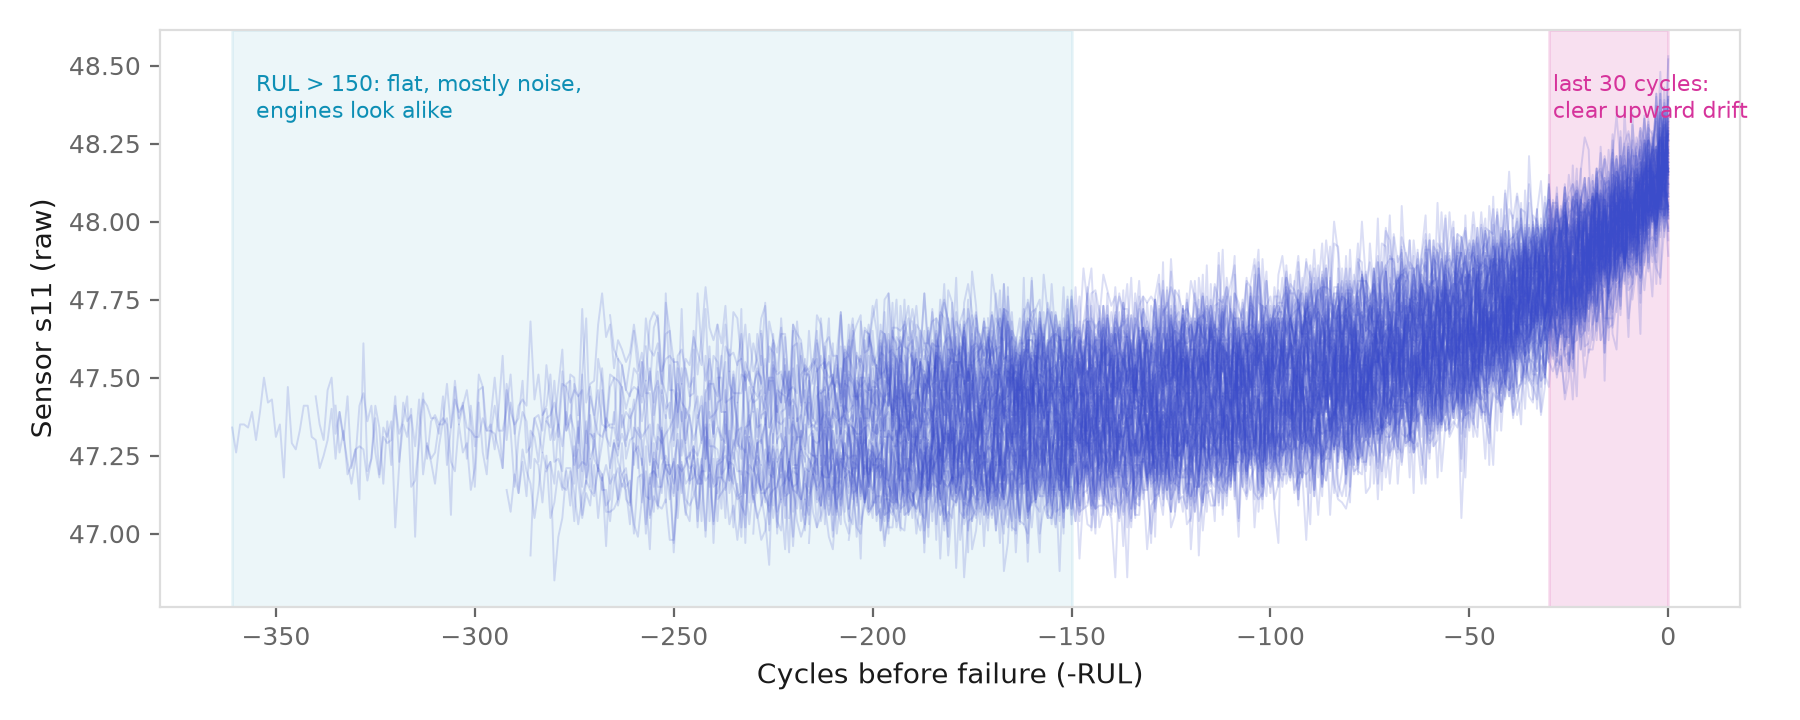
\includegraphics[width=\columnwidth]{figures/phase2_s11_all_engines.png}
\caption{Sensor s11 for all 100 training engines against cycles before failure.}
\label{fig:s11}
\end{figure}

\section{Methodology}
\subsection{Sequence windows}
For each row (engine $e$, cycle $t$) the input is the window $x_{t-W+1},\dots,x_t$ of the 14 sensors of engine $e$, with $W=30$. When $t<W$, the missing cycles are filled by repeating the engine's first reading. Windows never cross engines and contain nothing after $t$; both properties are checked by assertions in the notebook. Padding means every row still receives a prediction, so cross-validation is scored on the same 20{,}631 rows as in Phase 1 (Fig.~\ref{fig:windows}). $W=30$ is below the shortest test history (31 cycles), so every test engine has a full window of real readings at its last cycle. Sensors are z-scored with the mean and standard deviation of the training engines in each fold.

\begin{figure}[t]
\centering
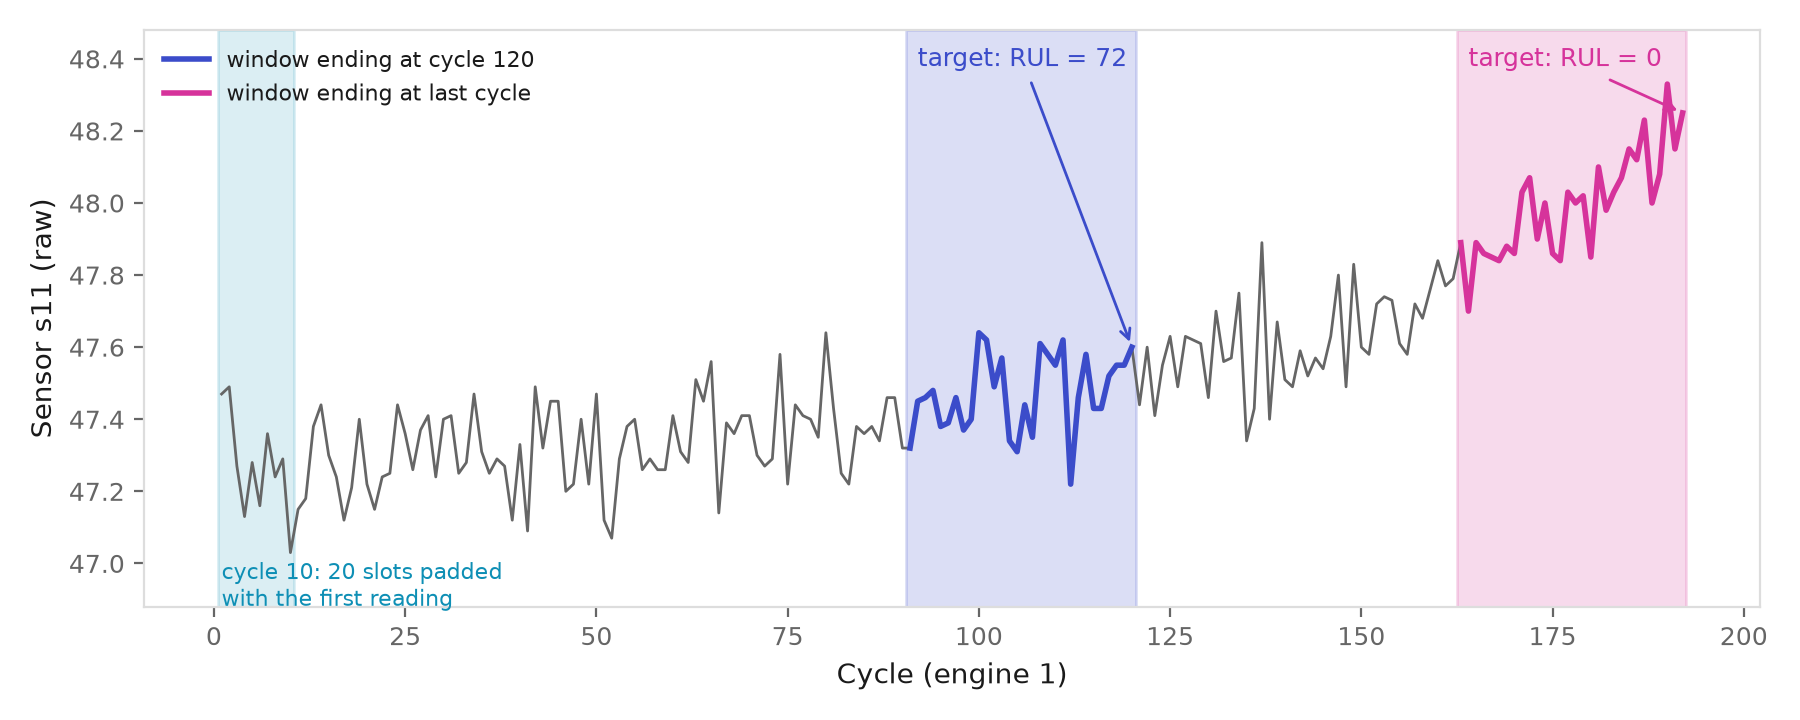
\includegraphics[width=\columnwidth]{figures/phase2_windows.png}
\caption{Two 30-cycle windows of sensor s11 for engine 1 and their targets. The shaded region at the start shows cycles that need padding.}
\label{fig:windows}
\end{figure}

\subsection{Models}
All models share a regression head (linear layer to 32 units, ReLU, dropout, linear layer to one output) and predict $\mathrm{RUL}/100$; predictions are multiplied by 100 and clipped at zero for scoring. Dividing by 100 only rescales the target and does not cap it.
\begin{itemize}
\item \textbf{LSTM} (main model, 55{,}873 parameters): two stacked LSTM layers with 64 hidden units and dropout 0.2 between them. The hidden state at the last time step feeds the head.
\item \textbf{Temporal CNN} (14{,}689): two 1D convolutions over time (kernel 5; 32 and 64 channels) followed by global average pooling. It tests whether recurrence matters.
\item \textbf{MLP} (5{,}825): a 64-unit layer on the 57 Phase 1 features at the current row. A control that sees no sequence.
\item \textbf{Hybrid} (57{,}697): the LSTM's last hidden state concatenated with the 57 standardised Phase 1 features (121 values) before the head (Fig.~\ref{fig:arch}).
\end{itemize}
The hybrid is motivated by Phase 1. There, the cycle number had an impurity importance of 0.559 and the health features compare each reading with the engine's first ten cycles. A 30-cycle window can see neither the engine's age nor its healthy baseline. The hybrid provides that long-term context alongside the learned short-term dynamics.

\begin{figure}[t]
\centering
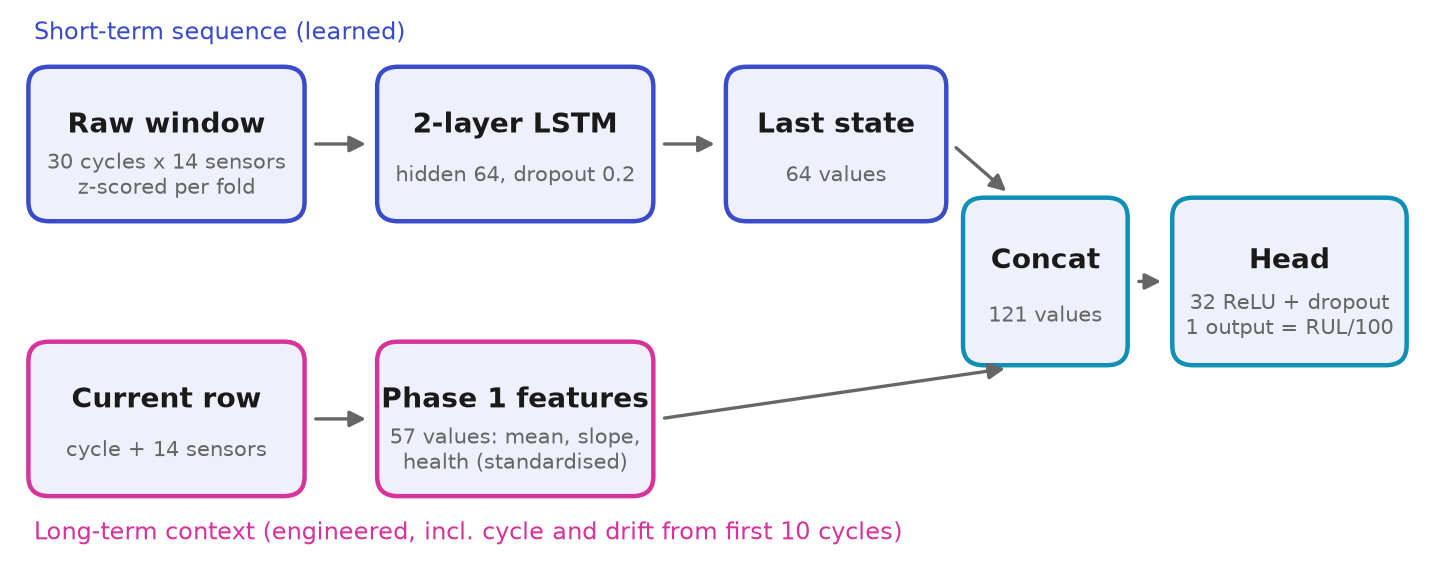
\includegraphics[width=\columnwidth]{figures/phase2_hybrid_architecture.png}
\caption{Hybrid model. The LSTM summarises the recent window; the engineered features add long-term context.}
\label{fig:arch}
\end{figure}

\subsection{Training and evaluation}
The outer loop is the Phase 1 protocol: 5-fold \texttt{GroupKFold} on engine ID, with identical row order and therefore identical folds, so each held-out engine is predicted exactly once. Inside each training fold, every fifth engine (16 engines) is held back to choose the early-stopping epoch, so the outer held-out engines are never used for any decision. Scalers are fitted on the remaining 64 engines. We train with Adam (learning rate $10^{-3}$, weight decay $10^{-4}$), batch size 256, mean squared error loss, gradient-norm clipping at 1.0 and at most 40 epochs, and stop when validation RMSE has not improved for 6 epochs, restoring the best weights. Hyperparameters are fixed defaults and were not tuned, as in Phase 1.

Metrics are RMSE and MAE in cycles, with MAE also reported for early (true RUL $\ge 50$) and late (true RUL $<50$) rows. For the test set, each model is retrained on all 100 training engines for the median best epoch from its cross-validation runs, using seeds 42, 43 and 44, and scored once at each test engine's last cycle. The Phase 1 Random Forest (200 trees, minimum leaf size 5) is re-run on the same folds as a reference. Its scores (cross-validation RMSE 35.17, test RMSE 23.32) differ slightly from the Phase 1 report (34.78 and 23.34) because of a different scikit-learn version.

\section{Results}
\subsection{Cross-validation and ablations}
Table~\ref{tab:cv} lists all cross-validation results; each ablation changes one setting relative to the main LSTM.

\begin{table*}[t]
\centering
\caption{5-fold grouped cross-validation on the 100 training engines, scored on uncapped RUL (mean $\pm$ std over folds, cycles).}
\label{tab:cv}
\begin{tabular}{llcccc}
\toprule
Model & Change from main LSTM & RMSE & MAE & MAE early & MAE late \\
\midrule
Random Forest (Phase 1) & 57 features, no network & 35.17 $\pm$ 1.52 & 23.03 $\pm$ 1.23 & 28.80 $\pm$ 1.47 & 5.02 $\pm$ 0.52 \\
\midrule
LSTM, $W=30$ (main) & -- & 41.76 $\pm$ 1.70 & 29.81 $\pm$ 2.00 & 35.40 $\pm$ 1.76 & 12.33 $\pm$ 3.97 \\
LSTM, $W=10$ & window length & 43.12 $\pm$ 0.99 & 31.10 $\pm$ 1.74 & 36.70 $\pm$ 1.49 & 13.60 $\pm$ 3.48 \\
LSTM, $W=50$ & window length & 41.61 $\pm$ 3.02 & 29.66 $\pm$ 3.57 & 35.26 $\pm$ 3.37 & 12.18 $\pm$ 4.91 \\
LSTM, no dropout & regularisation & 40.89 $\pm$ 3.59 & 29.86 $\pm$ 2.97 & 35.20 $\pm$ 3.22 & 13.14 $\pm$ 3.30 \\
Temporal CNN & architecture & 44.06 $\pm$ 3.56 & 31.69 $\pm$ 2.40 & 36.97 $\pm$ 2.86 & 15.19 $\pm$ 3.30 \\
MLP on 57 features & input: features only & 34.20 $\pm$ 3.27 & 22.03 $\pm$ 1.40 & 27.41 $\pm$ 1.74 & 5.23 $\pm$ 0.60 \\
Hybrid LSTM + features & input: window + features & 35.05 $\pm$ 2.19 & 23.76 $\pm$ 1.16 & 29.45 $\pm$ 1.39 & 6.00 $\pm$ 0.58 \\
Hybrid, capped at 125 & training target & 46.02 $\pm$ 1.81 & 27.72 $\pm$ 0.44 & 35.44 $\pm$ 0.57 & 3.60 $\pm$ 0.20 \\
\bottomrule
\end{tabular}
\end{table*}

\textbf{Raw windows versus features.} The raw LSTM is 6.6 cycles worse in RMSE than the Random Forest, more than the fold standard deviation of either model, and its late-stage MAE is more than twice as large (12.33 versus 5.02). Compared with the Phase 1 Elastic Net (cross-validation RMSE 40.04, late MAE 23.35, from the Phase 1 run), the LSTM is no better overall but much better near failure, so it does learn degradation from the raw signals.

\textbf{Window, dropout and architecture.} A 10-cycle window is worse than 30 or 50; 30 and 50 differ by 0.15 cycles, well within noise, so we keep 30. Removing dropout (40.89) and replacing the LSTM with a CNN (44.06) both change RMSE by less than the fold standard deviation (3.59 and 3.56). None of these settings closes the gap to the engineered features.

\textbf{Hybrid and control.} Adding the 57 features reduces RMSE from 41.76 to 35.05 and late-stage MAE from 12.33 to 6.00, bringing the hybrid level with the Random Forest. The MLP on the features alone, however, scores 34.20. The hybrid's improvement is therefore explained by the features; the LSTM branch adds no measurable value on top of them in this setting.

\textbf{Capping.} Trained on RUL capped at 125 and scored on the true RUL, the hybrid's RMSE rises to 46.02, because it cannot predict above 125 early in life. It has the lowest late-stage MAE of all models (3.60), which explains why capping is popular when the end of life is the main concern. This repeats the Phase 1 finding for the Random Forest.

\subsection{Training behaviour}
The raw LSTM reached its best validation score after 1 to 6 epochs in every fold. Training error keeps falling while validation error is flat or rising after the first epochs (Fig.~\ref{fig:curves}). Early in life, many windows look alike while their RUL differs by more than 100 cycles, so the network fits the training engines without learning a rule that transfers to new ones. Early stopping limits the damage.

\begin{figure*}[t]
\centering
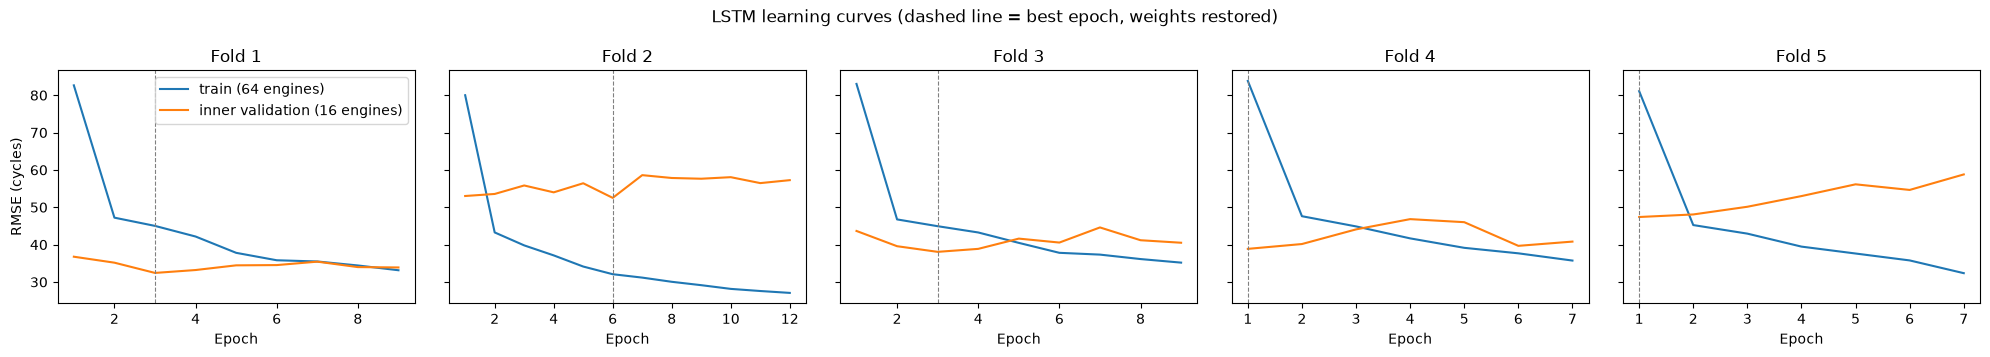
\includegraphics[width=0.95\textwidth]{figures/nb_learning_curves.png}
\caption{LSTM learning curves for each outer fold (train: 64 engines, inner validation: 16 engines). The dashed line marks the restored best epoch.}
\label{fig:curves}
\end{figure*}

\subsection{Error by degradation stage}
Fig.~\ref{fig:err} breaks the out-of-fold error down by true RUL. For RUL below 25 the MAE is 3.0 (Random Forest), 4.0 (hybrid) and 6.8 (raw LSTM); for 25 to 50 it is 7.4, 8.3 and 18.5. Between 125 and 175 cycles all three are similar, with the raw LSTM slightly ahead (21.0 versus 25.9 for the Random Forest in the 125--150 range). Above 200 cycles every model under-predicts heavily, as the scatter plot of the hybrid shows: predictions level off below about 200 regardless of the true value.

\begin{figure*}[t]
\centering
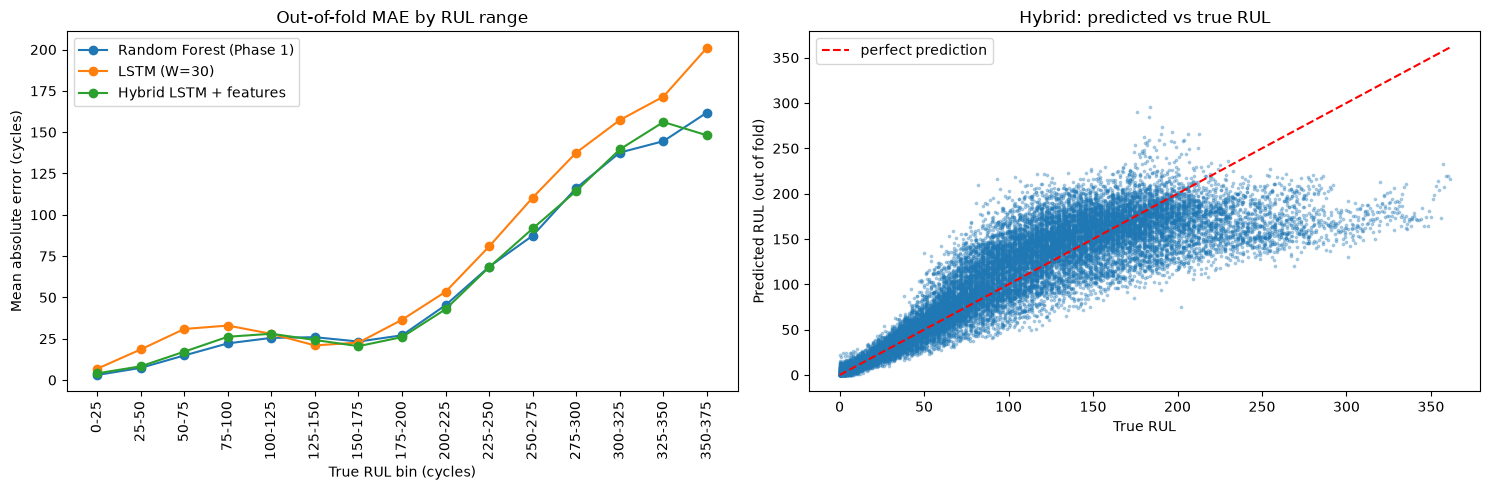
\includegraphics[width=0.9\textwidth]{figures/nb_error_analysis.png}
\caption{Out-of-fold MAE by true RUL range (left) and hybrid predictions against true RUL (right).}
\label{fig:err}
\end{figure*}

\subsection{Test set}
Table~\ref{tab:test} gives the single test evaluation. The MLP on engineered features has the lowest RMSE (21.59), followed by the Random Forest (23.32), the hybrid (25.23), the raw LSTM (25.33) and the CNN (26.27). Averaging the three seeds' predictions lowers RMSE slightly for every deep model (LSTM 24.29, CNN 25.27, MLP 21.30, hybrid 24.69). The raw LSTM varies strongly between seeds (standard deviation 3.55), consistent with its very short training (3 epochs). The hybrid is the most stable (0.15). On the 30 late test engines the Random Forest (4.03) and the hybrid (4.63) are most accurate. Fig.~\ref{fig:test} shows that all models track the true RUL closely for engines near failure and scatter by tens of cycles beyond about 60 cycles.

\begin{table}[t]
\centering
\caption{Test set, 100 engines at their last cycle. Deep models: mean $\pm$ std over 3 seeds.}
\label{tab:test}
\setlength{\tabcolsep}{3pt}
\resizebox{\columnwidth}{!}{%
\begin{tabular}{lcccc}
\toprule
Model & RMSE & MAE & Early MAE & Late MAE \\
\midrule
Random Forest & 23.32 & 15.57 & 20.52 & 4.03 \\
LSTM & 25.33 $\pm$ 3.55 & 18.29 $\pm$ 3.45 & 23.30 $\pm$ 4.44 & 6.58 $\pm$ 1.15 \\
CNN & 26.27 $\pm$ 0.74 & 19.89 $\pm$ 0.48 & 24.18 $\pm$ 0.22 & 9.87 $\pm$ 1.16 \\
MLP & 21.59 $\pm$ 0.44 & 14.91 $\pm$ 0.42 & 19.09 $\pm$ 0.39 & 5.15 $\pm$ 1.28 \\
Hybrid & 25.23 $\pm$ 0.15 & 17.68 $\pm$ 0.81 & 23.28 $\pm$ 0.91 & 4.63 $\pm$ 0.57 \\
\bottomrule
\end{tabular}}
\end{table}

\begin{figure}[t]
\centering
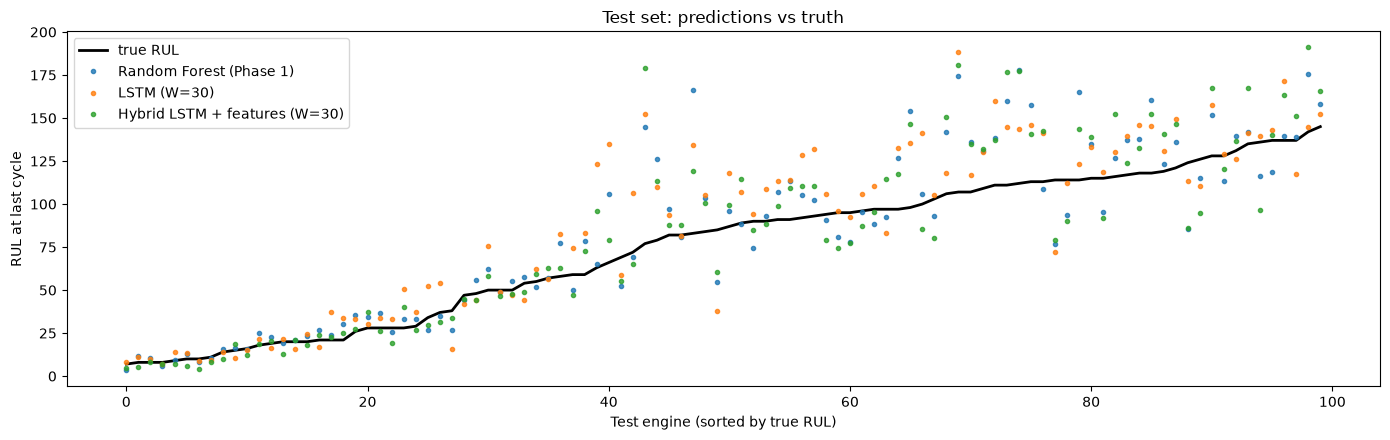
\includegraphics[width=\columnwidth]{figures/nb_test_predictions.png}
\caption{Test predictions at each engine's last cycle, sorted by true RUL (3-seed average for the deep models).}
\label{fig:test}
\end{figure}

\section{Discussion and Limitations}
The answer to the project question is clear on FD001 with an uncapped target: a 30-cycle raw window carries less usable information than the engineered features, and the deficit is in long-term context, not in model capacity. Changing the window, regularisation or architecture moves the raw model by less than the fold spread, while adding the engineered features moves it by 6.7 cycles. The hybrid idea is sound, since it supplies exactly the missing context, but the control experiment shows that the features alone do as well, so on this data the hybrid is not justified by results. The MLP's lower test RMSE than the Random Forest should not be read as a win: their cross-validation difference (34.20 versus 35.17) is within noise, and the test set has one cycle per engine.

Limitations: hyperparameters were not tuned, and ablations use a single seed and change one setting at a time; ablations reuse the comparison folds, so the best setting's score is slightly optimistic; padding the start of each engine with its first reading may let the network infer that a flat window means a young engine; the test score is noisy (100 engines, one cycle each); only FD001 is used; and the uncapped target makes our scores incomparable to most published work. Cross-validation and test scores measure different things, so their difference is not evidence about overfitting.

\section{Conclusion and Future Work}
Sequence models on raw 30-cycle windows learn real degradation signal (late-stage cross-validation MAE 12.33 for the LSTM) but do not match engineered features on the full uncapped RUL range (RMSE 41.76 versus 35.17). Combining the LSTM with the engineered features recovers the Random Forest's accuracy, yet an MLP on the features does as well, which points to long-term context as the key ingredient. Future work: sequences that cover each engine's full history so the network can see its healthy baseline, explicitly adding cycle number to the raw model, a capped target for end-of-life applications, a tuning search inside cross-validation, and the multi-condition subsets FD002 to FD004.

\begin{thebibliography}{20}
\bibitem{hochreiter1997lstm} S.~Hochreiter and J.~Schmidhuber, ``Long short-term memory,'' \emph{Neural Computation}, vol.~9, no.~8, pp.~1735--1780, 1997.
\bibitem{gers2000forget} F.~A.~Gers, J.~Schmidhuber, and F.~Cummins, ``Learning to forget: Continual prediction with LSTM,'' \emph{Neural Computation}, vol.~12, no.~10, pp.~2451--2471, 2000.
\bibitem{heimes2008rnn} F.~O.~Heimes, ``Recurrent neural networks for remaining useful life estimation,'' in \emph{Proc.\ Int.\ Conf.\ Prognostics and Health Management}, 2008.
\bibitem{zheng2017lstm} S.~Zheng, K.~Ristovski, A.~Farahat, and C.~Gupta, ``Long short-term memory network for remaining useful life estimation,'' in \emph{Proc.\ IEEE Int.\ Conf.\ Prognostics and Health Management (ICPHM)}, 2017, pp.~88--95.
\bibitem{babu2016cnn} G.~S.~Babu, P.~Zhao, and X.-L.~Li, ``Deep convolutional neural network based regression approach for estimation of remaining useful life,'' in \emph{Database Systems for Advanced Applications (DASFAA)}, 2016, pp.~214--228.
\bibitem{li2018cnn} X.~Li, Q.~Ding, and J.-Q.~Sun, ``Remaining useful life estimation in prognostics using deep convolution neural networks,'' \emph{Reliability Engineering \& System Safety}, vol.~172, pp.~1--11, 2018.
\bibitem{srivastava2014dropout} N.~Srivastava, G.~Hinton, A.~Krizhevsky, I.~Sutskever, and R.~Salakhutdinov, ``Dropout: A simple way to prevent neural networks from overfitting,'' \emph{J.\ Machine Learning Research}, vol.~15, pp.~1929--1958, 2014.
\bibitem{kingma2015adam} D.~P.~Kingma and J.~Ba, ``Adam: A method for stochastic optimization,'' in \emph{Proc.\ Int.\ Conf.\ Learning Representations (ICLR)}, 2015.
\bibitem{paszke2019pytorch} A.~Paszke \emph{et al.}, ``PyTorch: An imperative style, high-performance deep learning library,'' in \emph{Advances in Neural Information Processing Systems}, 2019.
\bibitem{saxena2008damage} A.~Saxena, K.~Goebel, D.~Simon, and N.~Eklund, ``Damage propagation modeling for aircraft engine run-to-failure simulation,'' in \emph{Proc.\ Int.\ Conf.\ Prognostics and Health Management}, 2008.
\bibitem{saxena2008cmapss} A.~Saxena and K.~Goebel, ``Turbofan engine degradation simulation data set,'' NASA Prognostics Data Repository, 2008.
\end{thebibliography}

\end{document}
